
\section{What happens when a discriminatively pretrained network is finetuned?}
\label{sec:fine}
%Finetuning a network is the process of slowly updating pre-learned parameters to minimize a target loss function for a new task at hand. Since, CNNs consist of large number of parameters they are prone to overfitting when trained on small datasets. Finetuning can be considered as a method of transfer learning and recent results from \cite{Rcnn, Decaf} presented a strong case for this methodology boosting performance. Although, unsupervised pretraining has been widely studied in the multilayer network literature \cite{AmitGeman, DeepPre}, there is no work analysing the effect of fine-tuning on different layers of a discriminatively trained multilayer convolutional networks.

%We start our analysis by investigating how the discriminative capacity of different layers of the network changes as a result of finetuning. We measure discriminative capacity using the entropy of each layer  
%We start our analysis by investigating how the entropy of filters across different layers changes as a result of discriminative fine-tuning (see sec \ref{sub:fine-entropy}). Since, entropy of a filter can be evaluated at different threshold level of activations we propose the metric of Area under the Entropy curve (AuE) to judge changes in filter selectivity. Our main finding is that most of the learning during finetuning happens only in the top two fully connected layers. Motivated by this observation, we finetune networks for PASCAL detection and SUN-397 scene classification task by setting non-zero learning rates only in the top 2 layers (see sec\ref{sub:fine-fc-only}). We find this results in a negligible drop in performance and allows for moderate speed-ups in finetuning time. Other conclusions are presented in the sec \ref{sub:fine-discussion}.

Results from \cite{Rcnn} suggested that fine-tuning a discriminatively pre-trained network is a powerful method for task specific feature learning. Consequently, we studied the effect fine-tuning on performance under the experimental setups of SUN-CLS and PASCAL-DET (section \ref{sub:effect-finetune}). We provide objective evidence that with less data, pre-training followed by fine-tuning is required for good performance, whereas with enough data, a CNN can be trained from scratch. We also find that fine-tuning with more data leads to better performance and this is used to establish the new state of art results on PASCAL-DET.

Given these results, it is important to understand the effect, fine-tuning has on the parameters of the CNN. Towards this end, we investigate the effect of fine-tuning for PASCAL-DET has on the discriminative capacity of individual features extracted from different layers of the CNN (section .) We find that discriminative capacity of individual features from layers 1 to 5 does not changes much, whereas features in layers 6 to 7 become substantially more discriminative. We use this observation to show that fine-tuning only the top two layers (i.e. 6,7) leads to as good performance as fine-tuning all layers on datasets of size PASCAL-DET and SUN-CLS. However, we also note that given larger datasets, fine-tuning only layers 6,7 is insufficient. This suggests that work such as (\todo{REF}) can benefit from fine-tuning all layers.        

\subsection{Effect of fine-tuning on performance}
\label{sub:effect-finetune}
\setlength{\tabcolsep}{2pt}
\begin{table}[t!]
\begin{center}
\caption{Comparing the performance of a CNN trained from scratch, pre-trained on Imagenet and fine-tuned for the particular task. VOC 2007 + 2012 data was used for training from scratch and fine-tuning for PASCAL-DET-2. }
\label{table:fine-effect}
\scalebox{0.9}{
\begin{tabular}{|l|ccc|ccc|ccc|}
\hline
Layer &  \multicolumn{3}{c|}{SUN-CLS} & \multicolumn{3}{c|}{PASCAL-DET} & \multicolumn{3}{c|}{PASCAL-DET-2} \\
\hline
  &    scratch & pre-train & fine-tune  & scratch & pre-train & fine-tune & scratch & pre-train & fine-tune\\
\hline
fc-7 & $40.2 \pm $ & $53.1 \pm 0.2$ & $56.8 \pm 0.2$ & 40.7 & 45.5 & 54.1 & 52.3 & 45.5 & 59.2 \\ 
\hline
\end{tabular}}
\end{center}
\end{table}
\setlength{\tabcolsep}{1.4pt}


\subsection{Effect of fine-tuning on network parameters}
\label{sub:fine-entropy}
We compute the entropy  curve of each filter (using the method described in \ref{sub:def-ent}) for all layers of Alex-Net and FT-Net using the ground-truth bounding boxes taken from the VOC-2007 test-set. 

We use Area under this entropy curve (AuE) to quantify selectivity of each filter. The distribution of AuE for all filters across the seven layers of the CNN is illustrated in fig \ref{fig:fine-hist}. Next, in order to determine the overall change in a layer's tuning we use the Cumulative AuE (C-AuE) of filters sorted in decreasing order of their individual AuE's. We normalize this metric appropriately to account for different number of filters in different layers. We call this normalized C-AuE as MC-AuE. A lower value of MC-AuE means that a layer is more selective.  Fig \ref{fig:fine-entropy} plots MC-AuE as a function of fraction of filters in each layer. 

\begin{figure}[t!]
\centering
\subfloat{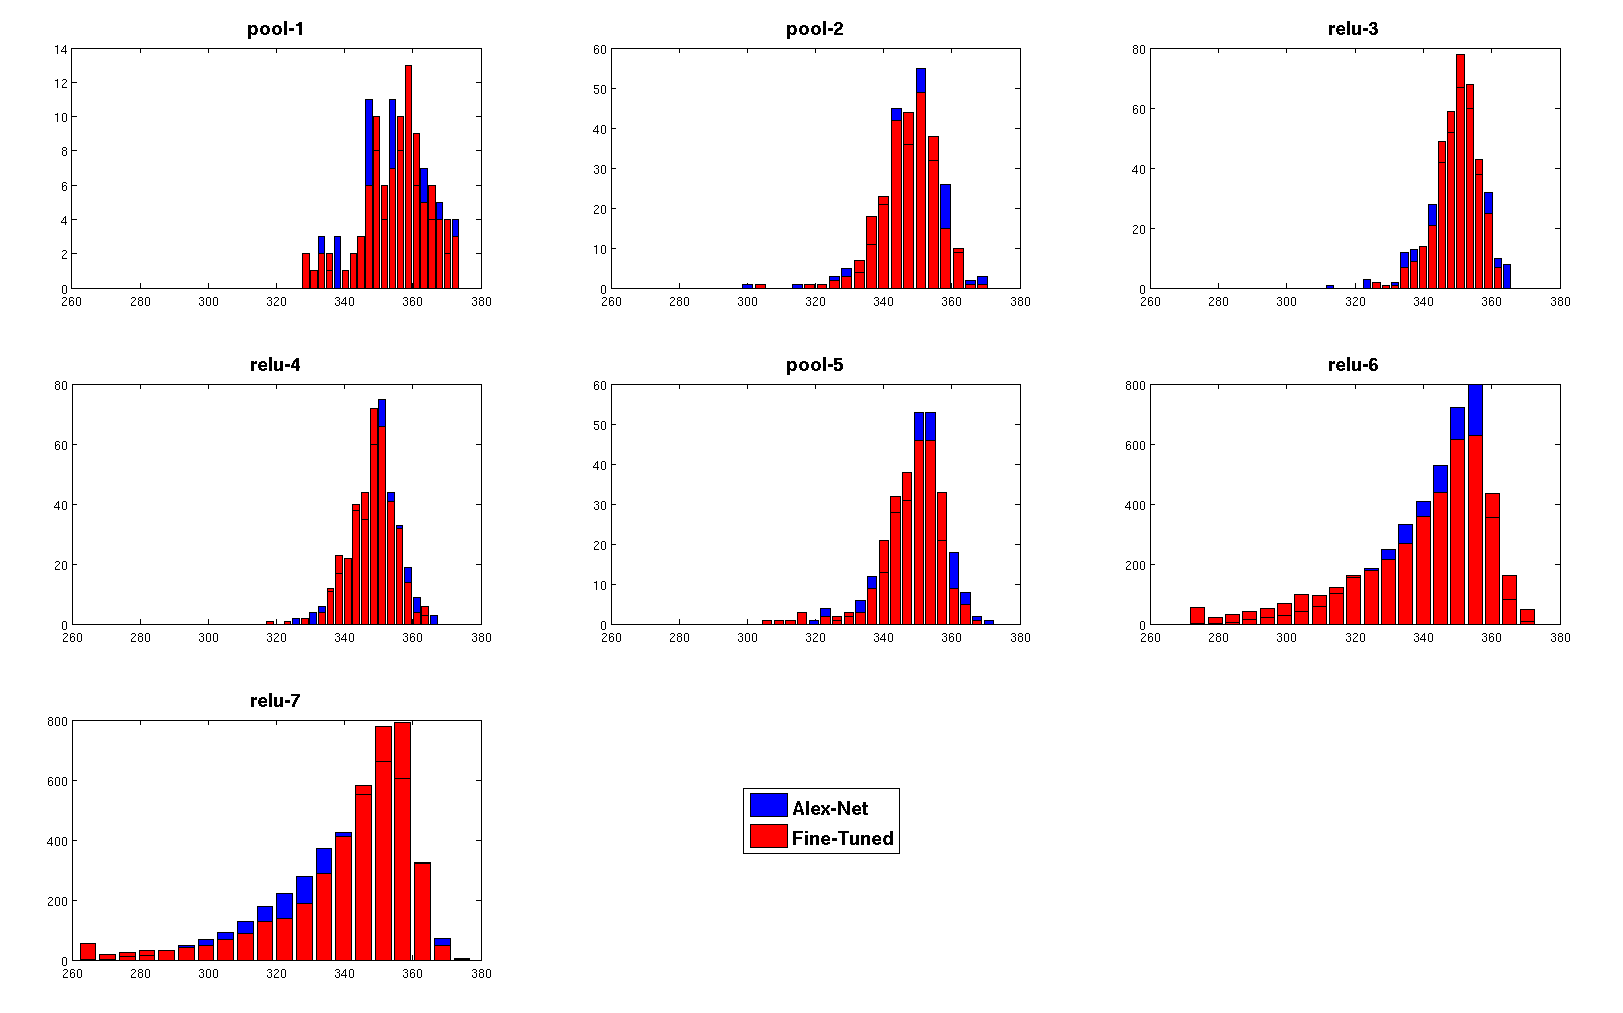
\includegraphics[height=6.5cm]{images/ent_hist.png}}
\caption{Distribution of AuE for different layers in Alex-Net and FT-Net. X-axis is the entropy and the Y-axis is the number of filters. Notice that the left tail for relu 6 and 7 becomes heavier after finetuning. This indicates that finetuning makes these filters more discriminative.}
\label{fig:fine-hist}
\end{figure}

\begin{figure}[t!]
\centering
\subfloat{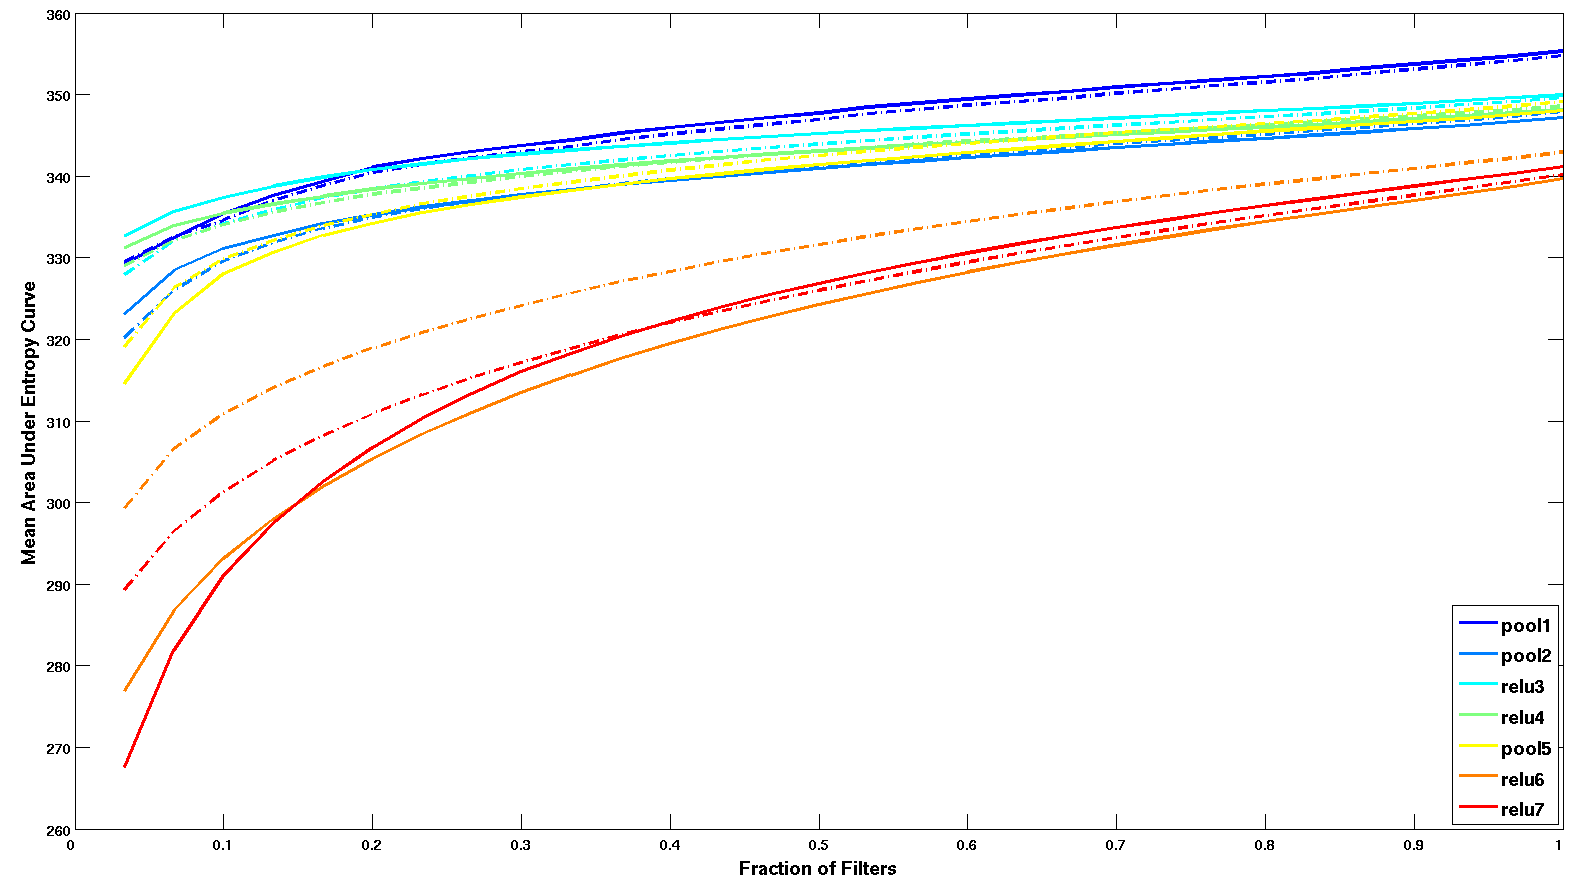
\includegraphics[scale=0.15]{images/entropy_variation.png}}
\caption{Mean Cumulative AuE plotted as fraction of filters (see sec \ref{sub:fine-entropy}). (Dash-Dot Line :Alex-Net, Solid Line: Fine-Tuned Network).}
\label{fig:fine-entropy}
\end{figure}

From figures \ref{fig:fine-hist} and \ref{fig:fine-entropy}, we draw 2 conclusions:
\begin{enumerate}
\item Although the entropy of filters decreases as we move to higher layers, the magnitude of change in entropy between layer 1 and layer 5 is small as compared to the change which happens when going from layer 5 to layer 6.
\item Finetuning mostly reduces the entropy of filters in the fully connected layers, there are small changes in layer 5 and negligible changes in other layers.
\end{enumerate} 

\subsection{Is finetuning only the fully-connected layers sufficient?}
\label{sub:fine-fc-only}
The observations made in \ref{sub:fine-entropy} indicate that finetuning the convolutional layers in the CNN may not be critical for achieving good-performance on novel datasets. We test this hypothesis on the 2 challenging tasks of object detection(PASCAL) and scene classification (SUN-397) by comparing the performance of a fully finetuned network with a network finetuned by only updating weights in the fully-connected (fc) layers. Our results are summarized in table \ref{table:fine-effect}.

\setlength{\tabcolsep}{2pt}
\begin{table}[t!]
\begin{center}
\caption{Comparison in performance on of Alex-Net, Finetuned Network(ft-net) and a network with only fc layers finetuned (fc-ft).}
\label{table:fine-effect}
\scalebox{0.85}{
\begin{tabular}{|l|cccc|cccc|cccc|}
\hline
Layer &  \multicolumn{4}{c|}{sun-397} & \multicolumn{4}{c|}{det VOC-2007-finetune} & \multicolumn{4}{c|}{det VOC-all-finetune} \\
\hline
  &    scratch & i-net & ft & fc-ft  & scratch & i-net & ft & fc-ft & scratch & i-net & ft & fc-ft\\
\hline
fc-7 & $40.2 \pm $ & $53.1 \pm 0.2$ & $56.8 \pm 0.2$ & $56.2 \pm 0.1$ & 40.7 & 45.5 & 54.1 & 53.3 & 52.3 & 53.1 & 56.0 & 59.2 \\ 
\hline
\end{tabular}}
\end{center}
\end{table}
\setlength{\tabcolsep}{1.4pt}

We find that indeed it is the case that the final performance in the detection setup only drops by 0.8 points and by 0.6 points for scene-classification. In our experiments we also noted accuracy of image classification on PASCAL is almost untouched by finetuning. This is suggestive of the fact finetuning is a task specific operation and finetuning for detection does not necessarily leads to an increase in classification performance, even though the classes and images are shared across PASCAL classification and detection challenges. 

\setlength{\tabcolsep}{1pt}
\begin{table}[t!]
\begin{center}
\caption{Evaluation of effect finetuning towards the task of object detection. (l5, l6, l7: layers 5, 6 and 7 of Alex Net)}
\label{table:det-fine}
\scalebox{0.75}{
\begin{tabular}{l|cccccccccccccccccccc||c}
\hline\noalign{\smallskip}
layer & aero & bike & bird & boat & bottle & bus & car & cat & chair & cow & table & dog & horse & mbike & person & plant & sheep & sofa & train & tv & mAP \\
\noalign{\smallskip}
\hline
l5 & 51.9 & 61.1 & 36.8 & 28.4 & 23.7 & 52.3 & 60.8 & 48.4 & 24.9 & 47.1 & 47.5 & 42.1 & 55.6 & 58.7 & 42.5 & 24.5 & 46.9 & 39.3 & 52.0 & 55.4 & 45.0 \\
l5-ft & 57.8 & 63.9 & 38.8 & 28.0 & 29.0&54.8&66.9&51.3 & 30.5 & 52.1 & 45.2 & 43.2 & 57.3 & 58.8 & 46.0 & 27.2 & 51.2 & 39.3 & 53.3 & 56.6 & 47.6 \\
\hline 
l6-ft &63.5 & 66.3 & 48.7 & 38.1 & 30.6 & 61.4 & 70.9 & 60.3 & 34.8 & 57.8 & 47.6 & 53.6 & 59.8 & 63.5 & 52.5 & 29.8 & 54.6 & 48.2 & 58.5 & 62.2 & 53.1 \\
l6-fc-ft& 61.4 & 63.9 & 44.2 & 36.2 & 29.0 & 59.9 & 66.0 & 55.3 & 31.1 & 57.6 & 49.5 & 49.4 & 59.4 & 63.7 & 50.8 & 29.5 & 54.1 & 43.2 & 57.4 & 58.8 & 51.0 \\
\hline
l7 & 57.6 & 57.2 & 41.4 & 31.2 & 25.6 & 52.4 & 58.8 & 50.9 & 25.2 & 50.4 & 42.7 & 47.1 & 52.2 & 55.6 & 44.5 & 23.9 & 48.0 & 38.1 & 51.5 & 56.6 & 45.5 \\
l7-ft & 64.3 & 69.6 & 50.1 & 41.8 & 32.0 & 62.6 & 71.0 & 60.6 & 32.8 & 58.5 & 46.4 & 56.0 & 60.0 & 66.9 & 54.2 & 31.5 & 52.7 & 48.8 & 57.7 & 64.7 & 54.1 \\
l7-fc-ft & 62.9 & 65.2 & 47.5 & 39.0 & 30.3 & 63.1 & 68.4 & 59.7 & 34.2 & 58.5 & 52.0 & 53.8 & 60.7 & 65.3 & 53.0 & 30.2 & 55.5 & 46.3 & 57.7 & 62.2 & 53.3 \\
\hline
\end{tabular}}
\end{center}
\end{table}
\setlength{\tabcolsep}{1.4pt}

A detailed layer-wise analysis of detection performance for all PASCAL classes and the 3 network configurations is presented in table \ref{table:det-fine}. Notice that for both the finetuned networks there is big jump in the performance while going from layer 5 to 6 and a rather small jump from layer 6 to 7. For Alex-Net, the performance is virtually the same for layers 5 and 7. It is also notable, that although the performance for FT-net is better by 2.6 points at layer 5 - the performance is virtually the same at layer 7. 
\subsection{Discussion}
\label{sub:fine-discussion}
Since layers 1-5 change a little over the course finetuning, this suggests that these are generic features. Although, one could always improve performance by a few points by finetuning the full network - for a lot of applications this may not be practical. 
It is also notable to point out that the more or less generic representations learnt in layer 4 and 5 are in contrast with some of the mid-level feature learning work such as \cite{Blocks} \cite{Mid1} wherein the problem of finding good mid-level parts is often posed as a greedy search for high recall discriminative templates.